\frame
{
\frametitle{\citetitle{8994792} (1)}

\begin{columns}
\column {0.9\textwidth} 
\begin{itemize}
\item Según la Organización para la Agricultura y la Alimentación (FAO), México es uno de los cinco principales productores de cítricos del mundo. 
\item Los productores de cítricos requieren máquinas clasificadoras capaces de
clasificar frutas según determinadas características (tamaño y color). 
\item La segmentación de imágenes es la primera etapa en una proceso de clasificación. 
\end{itemize}
 \column {0.1\textwidth} 
 \begin{center}
    %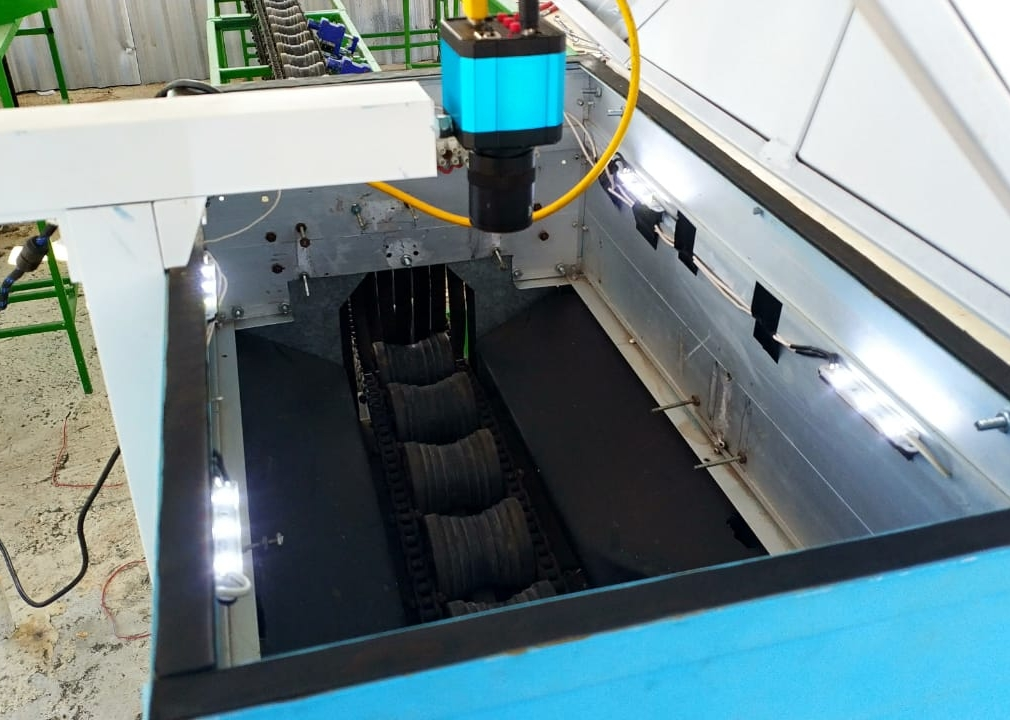
\includegraphics[width=0.9\textwidth]{Figs/2019_Naranjas_cabina}\\
    %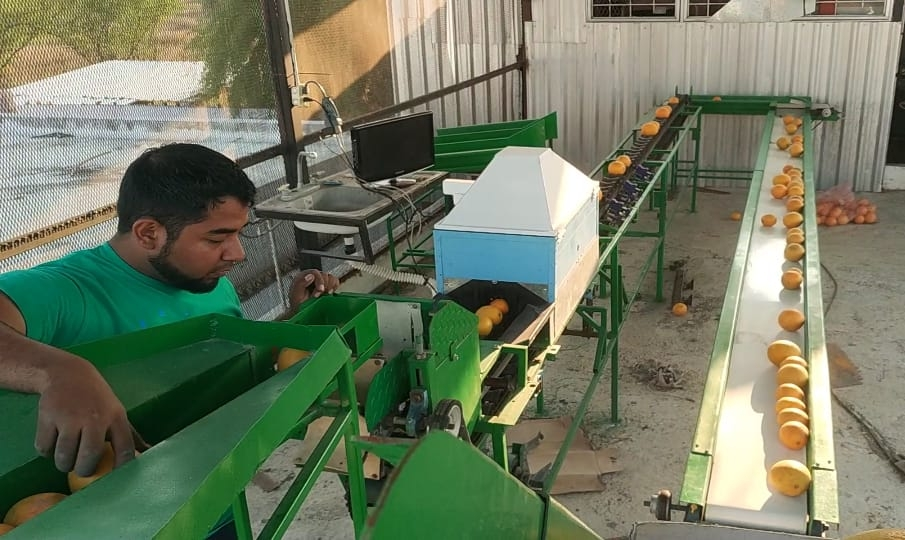
\includegraphics[width=0.9\textwidth]{Figs/2019_Naranjas_Maq}
 \end{center}
\end{columns}


\footnotetext[1]{\fullcite{8994792}}

}

\frame
{
\frametitle{Implementación}
\begin{columns}
 \column {0.5\textwidth} 
 \begin{itemize}
        \item En una primer etapa, se capturaron videos de naranjas pasando a través de la máquina
        \item A partir de esos videos, se propuso un algoritmo para segmentar las naranjas de acuerdo con el color de clasificación deseado
        \item A partir de las naranjas segmentadas, se propuso un modelo  
        \item Ese modelo fue puesto en operación.
 \end{itemize} 
%\begin{center} 
%    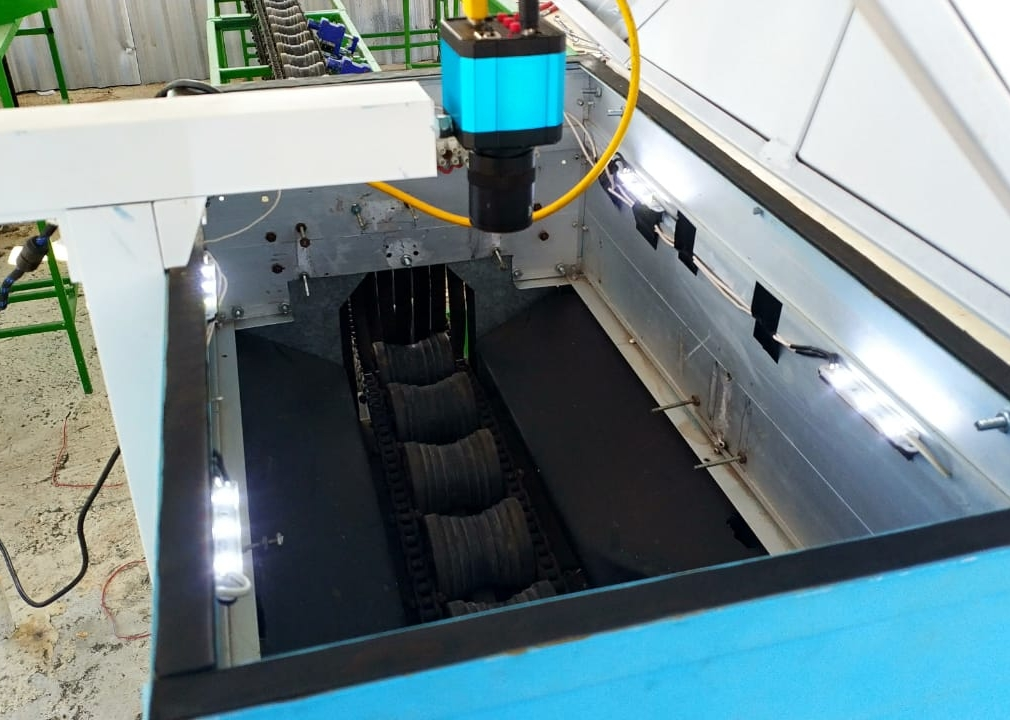
\includegraphics[width=0.7\textwidth]{Figs/2019_Naranjas_cabina}

%\end{center}     
 \column {0.5\textwidth} 
 \begin{center}
    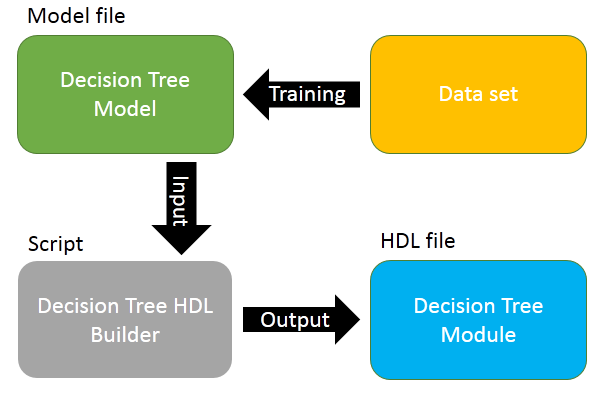
\includegraphics[width=0.7\textwidth]{Figs/2019_Naranjas_weka_overview1}\\
    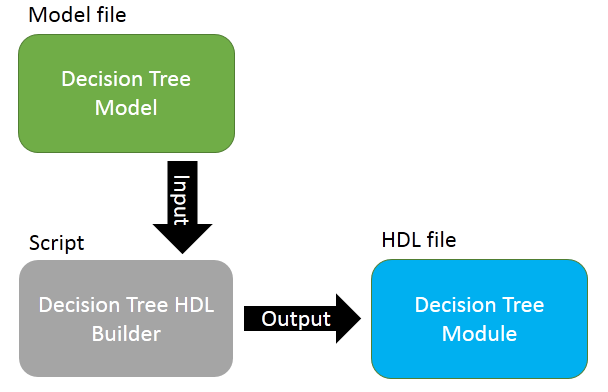
\includegraphics[width=0.7\textwidth]{Figs/2019_Naranjas_weka_overview2}
   \end{center}
\end{columns}


}

\frame
{
\frametitle{Resultados}
\begin{columns}
 \column {0.5\textwidth} 
    \begin{itemize}
        \item Se utilizó una tarjeta Industrial Video Processing Kit (Avnet).
        \item Incluye entrada de video HDMI.
        \item El rendimiento máximo del sistema propuesto es de una tonelada de fruta en 18 minutos.
    \end{itemize}         
 \column {0.5\textwidth} 
 \begin{center}
    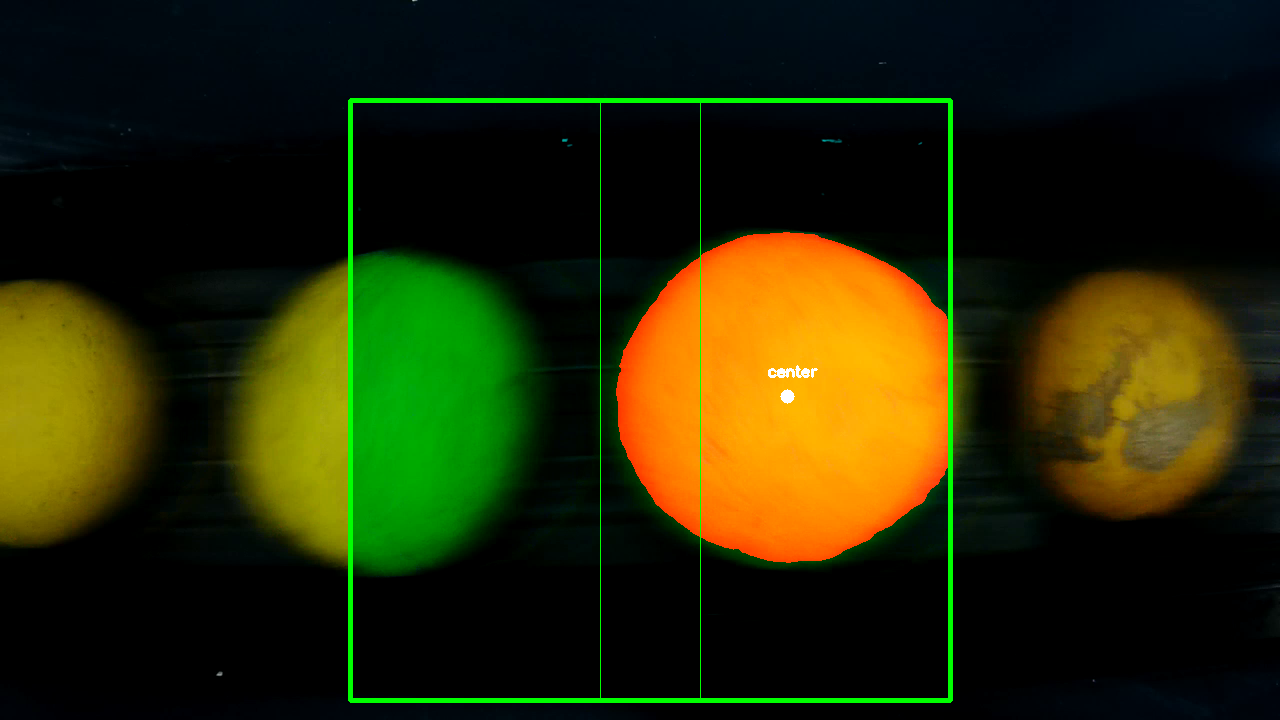
\includegraphics[width=0.7\textwidth]{Figs/2019_Naranjas_Segmentation1}\\
    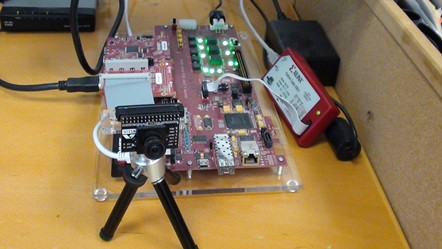
\includegraphics[width=0.7\textwidth]{Figs/2019_Naranjas_Industrial_Video_Processing_Kit}
   \end{center}
\end{columns}
}
